\documentclass{beamer}

\mode<presentation>
{
\usetheme{Dresden}

\setbeamercovered{transparent}
}

\usepackage[english]{babel}
\usepackage[latin1]{inputenc}
\usepackage{amsfonts}
\usepackage{amsmath}
\usepackage{mathtools}
\usepackage{listing}
\usepackage[scaled=.90]{helvet}
\usepackage{courier}
\usepackage{graphicx}
\usepackage{color}
\usepackage{subfig}
\DeclareGraphicsExtensions{.pdf,.png,.jpg,.mps}
\usepackage[absolute,overlay]{textpos}
\setlength{\TPHorizModule}{1mm}
\setlength{\TPVertModule}{1mm}
\usepackage{ragged2e}
\justifying
\usepackage{color}
\usepackage{physics}
\usepackage{mathtools}
\usepackage{amsmath}
\usepackage{bm}
\usepackage{calc}
\usepackage{listings}
\usepackage{url}
\usepackage{rotating}
%\usepackage{calrsfs}
\usepackage{amsfonts}
\usepackage[T1]{fontenc}

%%%% A NEW COMMAND TO FIX LOGO POSITION (x,y) in mm
\newcommand{\MyLogo}{%
\begin{textblock}{13}(88,74)
%  \pgfuseimage{logo}
 
\includegraphics[height=1cm, angle=0]{images/pdp2017}
\end{textblock}
} 


%%%% A NEW COMMAND TO FIX LOGO POSITION (x,y) in mm

%%%%%%%%%%%%%%%%%%%%%%%%%%%%%%%%%%%%%%%%%%%%%%%%%%%%%%%%%%%%%%%%%%%%%%%%%

\title{A Tracking Algorithm for Particle-like Moving Objects}

\author{Davide Spataro, Paola Arcuri, Alessio De Rango, William Spataro, Donato D'Ambrosio\inst{1} and Alice Mari\inst{2}}
\institute[]{\inst{1} University of Calabria, Department of Mathematics and Computer Science \and %
\inst{2} Institute for BioEngineering University of Edinburgh}
\date{PDP 2017,  St. Petersburg, Russia\\
March 5-8, 2017}

\begin{document}

\begin{frame}
\MyLogo
\MyLogo
\titlepage
\end{frame}


\begin{frame}{Contents}
\tableofcontents
\end{frame}


\section{Introduction}
%Frame----------------------------------------------------------------------------------------------------------------------------------------------------
	\begin{frame}{Motivations}
				\begin{itemize}
					\item How bacteria react to a stimulus
					\item How a drug interfere with bacteria, changing their chemiotaxis i.e. change in movements
					\item For example monitoring how good is a drug impeding communication between cancer cells.
					\item When the number of \textit{particles} is high, manual evaluation is \textbf{infisable}
				\end{itemize}
				


	\end{frame}
	
	%Frame----------------------------------------------------------------------------------------------------------------------------------------------------
		\begin{frame}{Motivations}
				\begin{figure}
					\centering
					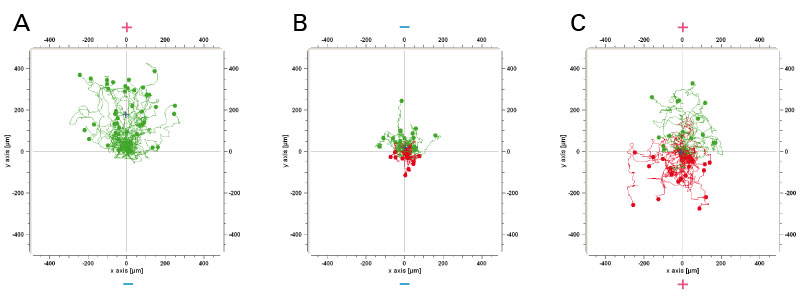
\includegraphics[scale=0.38]{./images/motivations.png}
				\end{figure}

				\begin{itemize}
					\item A: \textit{Normal} trajectories
					\item B: Drug is administred
					\item C: Red trajectories are of those who were affected by the drug
				\end{itemize}
				\textbf{Tracking allows  quantitatively analysis}!
	\end{frame}
	
%Frame----------------------------------------------------------------------------------------------------------------------------------------------------
		\begin{frame}{Motivations}
				\begin{figure}
					\centering
					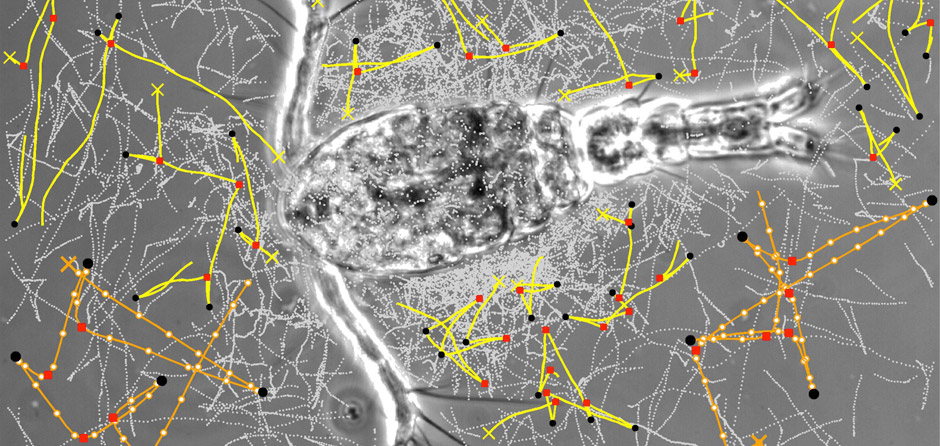
\includegraphics[scale=0.30]{./images/motivations2.png}
				\end{figure}

				\begin{itemize}
					\item spiega che è sta cosa
				\end{itemize}

	\end{frame}
	
	
	%Frame----------------------------------------------------------------------------------------------------------------------------------------------------
		\begin{frame}{Motivations}
				\begin{figure}
					\centering
					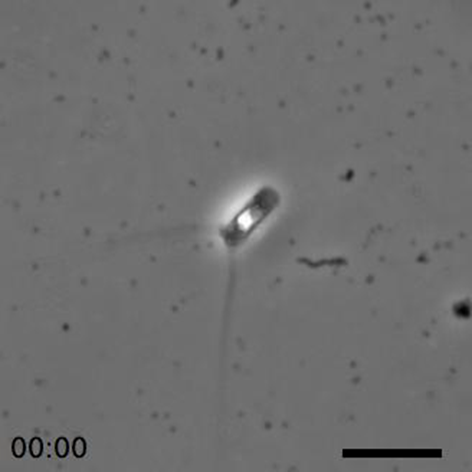
\includegraphics[scale=0.30]{./images/motivations3.png}
				\end{figure}

				\begin{itemize}
				\item alga che muore e rilascia i nutrienti de quei cosi piccoli sono i batteri che si muovo per magnare
				\end{itemize}

	\end{frame}
	
	

\section{Tracking Algorithm}

	\subsection{Image Processing Using XCA}
%Frame----------------------------------------------------------------------------------------------------------------------------------------------------
		\begin{frame}{XCA - IFCA Engine - CA}
			\begin{itemize}
			\item Cellular Automata (CA) are \textbf{Turing complete dunamical system} and also a \textbf{parallel computational models} (\textit{von Neumann 1966})
			\item CA can be described as a matrix of simple processing units, the cells, each one interacting with its neighbouring ones

			\end{itemize}
					\begin{figure}
					\centering
					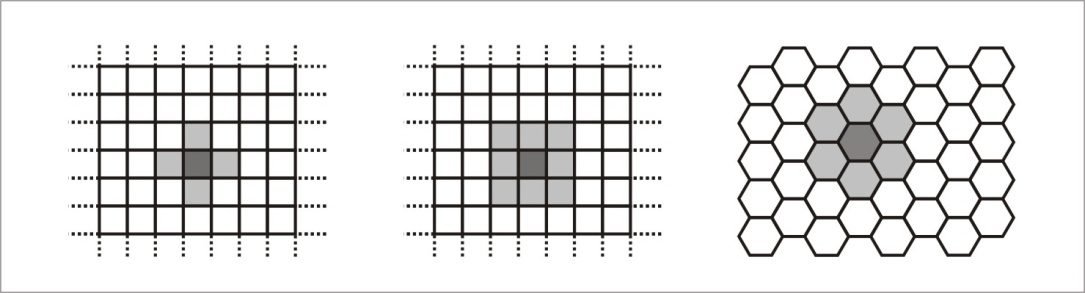
\includegraphics[scale=0.68]{./images/CA}
				\end{figure}
		\end{frame}
%Frame----------------------------------------------------------------------------------------------------------------------------------------------------
		\begin{frame}{XCA - IFCA Engine - CA}
		\[
			A = \Big<Z^d , Q, X, \tau \Big>		
		\] where:
		\begin{itemize}
		 \item $Z^d$ is the $d-$dimensional Cellular Space.
		 \item $Q$ is the \textbf{finite} set of states of the cell
		 \item $X = \{\xi_0, \xi_1, \ldots , \xi_{m-1}\}$ is the finite set of $d-$dimensional vectors that define the set of coordinates of the neighbouring cells $V(X,i)=\{i+\xi_0, i+\xi{1},\ldots, i+\xi{m-1}\}$

		 \item $\tau: Q^m \mapsto  Q$ is the deterministic transition function for the cell. $tau$ is applied simultaneously to each cell, for each CA step
		\end{itemize}
		\end{frame}
		
%Frame----------------------------------------------------------------------------------------------------------------------------------------------------
		\begin{frame}{XCA - IFCA Engine }
\begin{block}{A (farly large) number of Image Processing algorithm can be expressed as CA}
Convolutional filters $\mapsto$ $X$ and $\tau$ in CA's world.

\end{block}		
		
		\begin{figure}
					\centering
					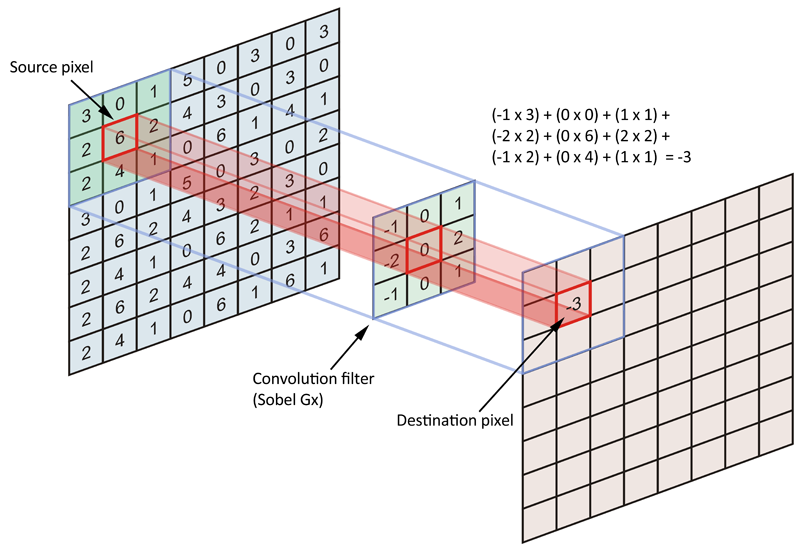
\includegraphics[scale=0.28]{./images/kernel_convolution}
				\end{figure}
		\end{frame}	

%Frame----------------------------------------------------------------------------------------------------------------------------------------------------
		\begin{frame}{XCA - IFCA Engine }
\begin{block}{Use CA instead of normal IP tecniques to get parallelism transparently!}
\end{block}		
		

		\begin{itemize}
			\item Implemented on top of \textbf{OpenCAL}
			\item Each color channels is represented as a substate
			\item Local and Global Pixel transformations maps directly to \textit{elementary processes} and \textit{global operations}, respectively.
			\item Runs on a number of parallel architectures and accelerators
			\item Easy to use. Threshold Filter in ~$20$ LoC.
			\item Seamless input/output
			\end{itemize}
		\end{frame}
		%Frame----------------------------------------------------------------------------------------------------------------------------------------------------
		\begin{frame}[fragile]{XCA - IFCA Engine}
			 \begin{lstlisting}[language=C,basicstyle=\tiny\ttfamily]
template<uint DIM, class NEIGH, typename CT, class PT>
class ThresholdFilter : public opencal::CALLocalFunction< DIM , NEIGH , CT>{

    TYPE lowT , highT ;
    TYPE outRangeValue , inRangeValue;

    ThresholdFilter(auto* sbs, TYPE _lowT , TYPE _highT , TYPE _outrange, TYPE _inrange ):
        img(sbs), lowT(_lowT) , highT(_highT) , 
        outRangeValue(_outrange) , inRangeValue(_inrange) { }
    
    void run(MODELTYPE* model,std::array<CT,DIM>& indices){
        
        constexpr int channels = std::tuple_size<PT>::value;
        PIXELTYPE newVal=img->getElement(indices);

        for (int i = 0; i<channels; ++i){
            const TYPE output =  (newVal[i] >= lowT && newVal[i] <= highT) ?
            					 inRangeValue : outRangeValue ;
            newVal[i] = output;
        }
        img->setElement(indices,newVal);
    }
};			
			
	\end{lstlisting}
		\end{frame}		
		
	
%Frame----------------------------------------------------------------------------------------------------------------------------------------------------
		\begin{frame}{IFCA Engine - Example: $N-$Dimensional Laplacian Filter}
			
		\end{frame}	
		
	\subsection{Trajectories Reconstruction}	
%Frame----------------------------------------------------------------------------------------------------------------------------------------------------	
		\begin{frame}{Objective}
			\begin{block}{Algorithm}
				From a set of particle representations construct a set of trajectories over time.
			\end{block}
			
			
			
		\end{frame}
	%Frame----------------------------------------------------------------------------------------------------------------------------------------------------
%Frame----------------------------------------------------------------------------------------------------------------------------------------------------	
		\begin{frame}{Objective}
	
		\begin{figure}
					\centering
					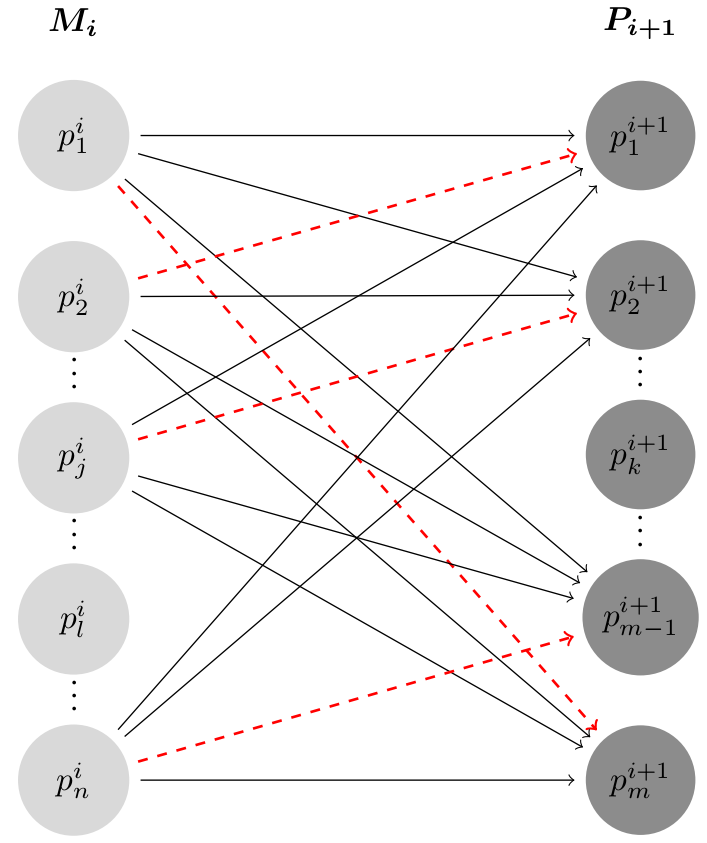
\includegraphics[scale=0.18]{./images/graph.png}
				\end{figure}
			
			
			
		\end{frame}

	


\section{Test Case: Motility of B. Subtilis}
%Frame----------------------------------------------------------------------------------------------------------------------------------------------------
	\begin{frame}{Experiment Setting}

	\end{frame}
%Frame----------------------------------------------------------------------------------------------------------------------------------------------------
	\begin{frame}{How Bacteria Moves?}

	\end{frame}
%Frame----------------------------------------------------------------------------------------------------------------------------------------------------




\begin{frame}%%     2
\begin{center}
{\fontsize{40}{50}\selectfont Thank You!}
\end{center}
\end{frame}

\end{document}